%--------------------
% Packages
% -------------------
\documentclass[11pt,a4paper]{article}
\usepackage[utf8]{inputenc}
\usepackage{fontenc}
\usepackage{amsmath}
\usepackage{graphicx}
\usepackage{subcaption}
%\usepackage{gentium}

\usepackage[english]{babel}
\usepackage[pdftex,linkcolor=black,pdfborder={0 0 0}]{hyperref} % Format links for pdf
\usepackage{calc} % To reset the counter in the document after title page
\usepackage{enumitem} % Includes lists

\frenchspacing % No double spacing between sentences
\linespread{0.9} % Set linespace
\usepackage[a4paper]{geometry} %margins
%\usepackage{parskip}

\usepackage[all]{nowidow} % Tries to remove widows
\usepackage[protrusion=true,expansion=true]{microtype} % Improves typography, load after fontpackage is selected


%-----------------------
% Set pdf information and add title, fill in the fields
%-----------------------
\hypersetup{ 	
pdfsubject = {CS698-P1},
pdftitle = {Speech Emotion Recognition},
pdfauthor = {Gaurav Sahu}
}

\title{\textbf{Speech Emotion Recognition}}
\author{Gaurav Sahu, MMath CS, University of Waterloo}
\date{\today}

%-----------------------
% Begin document
%-----------------------
\begin{document}

\maketitle
\section*{Abstract}

The aim of this project is to explore the domain of Speech Emotion Recognition (SER), i.e., automatically identifying human emotions from speech. It would be specifically helpful to use speech as it provides us with additional information that could aid ambiguity-resolution in communication. For example, ``I'm fine", could be said in multiple ways and we would not be able to identify the correct context if we only consider textual features. However, the task of SER is not trivial as the idea of ``emotion" is innately quite subjective and it could be a bit challenging for a machine to understand. Most of the works in literature focus on the ``big six" emotion-classes, namely, anger, disgust, fear, happiness, sadness, and neutral. In this work, we would be using the same and would especially focus on identifying emotion indicators using audio-based features such as pitch, loudness, and pause. More details about the approach and the dataset to be employed are described in the following sections.


\subsection*{Dataset and Preprocessing}
We would be using the following datasets for our experiments:

\begin{enumerate}
\item \textit{IEMOCAP:} The Interactive Emotional Dyadic Motion Capture Database (IEMOCAP) dataset \cite{busso2008iemocap} was released in 2008 by researchers in University of Southern California (USC). It contains five recorded sessions of conversations from ten speakers and amounts to 12 hours of audio-visual information. It is annotated with categorical emotion labels (Anger, Happiness, Sadness, Neutral, Surprise, Fear, Frustration and Excited) and dimensional labels (values of the activation and valence from 1 to 5).

%\item \textit{Berlin Database of Emotional Speech \cite{burkhardt2005database}:} This dataset was released in 2005 and contains 500 utterances spoken by 111 actors. It contains seven labels , namely, Neutral, Anger, Fear, Joy (Happiness), Sadness, Disgust and Boredom. Here, ``boredom" is an extra emotion type which we may use in addition to the ``big six" set of emotions.

\item \textit{SAVEE:} The Surrey Audio-Visual Expressed Emotion (SAVEE) dataset \cite{jackson2014surrey} was released in 2014 by researchers at the University of Surrey and consists of recordings from 4 male actors in 7 different emotions (anger, disgust, fear, happiness, sadness, neutral and surprise), 480 British English utterances in total. It also comes with text annotations with 15 sentences per emotion: 3 common, 2 emotion-specific and 10 generic.
\end{enumerate}

The SAVEE dataset was straightforward to deal with as it contained short wav files with their respective annotations. However, the IEMOCAP dataset provides wav files for individual sessions. So each of the session-specific wav files were segmented into shorter files in order to construct a corpus aptly aligned with its annotations. Finally, all the wav files were trimmed to remove the \textit{silent noise} from the audio.

\subsection*{Proposed Approach and Algorithms}
The task of SER is not new and has been studied for quite some time in literature. Recent introduction of deep neural networks to the domain has also significantly improved the state-of-the-art performance. In this work, we construct features from audio alone and observe what effects does it have when combined with textual features. We now describe some relevant features from the literature \cite{ververidis2006emotional} for our \textit{audio-only} framework and respective algorithms to compute them:

\begin{enumerate}
\item \textbf{Pitch:} Pitch is important because wave forms produced by our vocal cords change depending on our emotion. Many algorithms for estimating the pitch signal exist. We will use the most common method based on \textit{autocorrelation of center-clipped} frames \cite{sondhi1968new}.


Formally, the input signal $y[n]$ is center-clipped to give a resultant signal, $y_{clipped}[n]$, given by:


\[
y_{clipped}[n]= 
\begin{cases}
y[n] - C_l,& \text{if } y[n]\geq C_l\\
0,              & \text{if } |y[n]| < C_l\\
y[n] + C_l, & \text{if } y[n] \leq C_l
\end{cases}
\]

Here, $C_l$ is nearly half the mean of the input signal and $[\cdot]$ denotes that the input signal is discrete in nature. Now, autocorrelation is calculated for the obtained signal $y_{clipped}$, which is further normalized and finally the peak values are taken and associated with the pitch of the given input $y[n]$. It was found that center-clipping the input signal resulted in more distinct autocorrelation peaks.

\item \textbf{Number of Harmonics:} In the emotional state of anger or for stressed speech, there are additional excitation signals other that pitch (\cite{teager1990evidence}, \cite{zhou2001nonlinear}). This additional excitation is apparent in the spectrum as harmonics and cross-harmonics (Also shown by \ref{fig:harm_rmse}(a)). Harmonic calculation is based on the algorithm described in \cite{fitzgerald2010harmonic}


\item \textbf{Speech Energy:} This feature is related to the loudness in speech and hence, can be used for emotion recognition (See \ref{fig:harm_rmse} (b) for reference). We use the standard Root Mean Square Energy (RMSE) to calculate the signal given by:

\begin{equation}
	E = \sqrt{\frac{1}{n}\sum_{i=1}^{n} y[i]^{2}}
\end{equation}

\item \textbf{Pause:} This feature represents the ``silent" portion in the audio data. This quantity is directly related to our emotions; For example, we tend to speak very fast (resulting in low value of the feature) when excited (say, angry or happy). In order to calculate this value, we set a manual threshold $t = 0.4*E$ and the feature value is give by the probability $P(y[n]) < t$.
\end{enumerate}

Apart from the features described above, some other statistical metrics such as mean and standard deviation of the input signal have been used as features too.

All the pre-processing

\subsection*{Evaluation Measures and Next Steps}


Now that we have extracted features from audio samples, the next steps would be to:

\begin{enumerate}
\item Train a multi-class classifier (such as SVM, Random Forest, and Gradient Boosting)
\item Implement the \textit{text-only} baseline sequence-to-sequence architecture \cite{sutskever2014sequence} with attention mechanism \cite{bahdanau2014neural} and evaluate it against the available transcriptions
\item Combine features from both text and audio and observe the effect in performance
\item Implement the current state-of-the-art for multi-modal sentiment classification \cite{liu2018efficient} and compare its performance with that of the proposed model's
\end{enumerate}

We will use classification accuracy as the primary criterion for evaluation; However, accuracy could be sometimes misleading and hence we would also calculate a more normalized metric, the F-score, which is defined the harmonic mean of precision and recall.

\begin{figure}[h!]
	\centering
	\begin{subfigure}[b]{0.4\linewidth}
		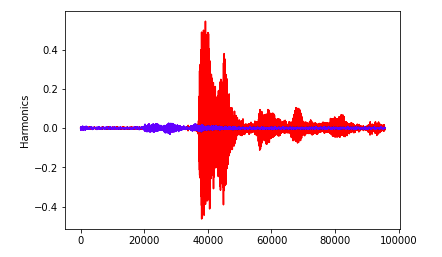
\includegraphics[width=\linewidth]{pictures/harmonics.png}
		\caption{Harmonics of angry (red) and sad (blue) audio signals}
	\end{subfigure}
	\begin{subfigure}[b]{0.4\linewidth}
		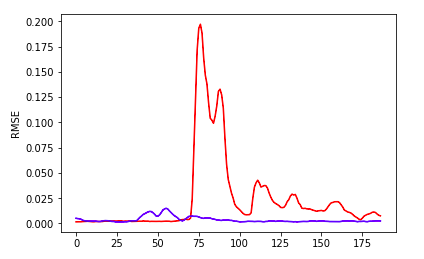
\includegraphics[width=\linewidth]{pictures/rmse.png}
		\caption{RMSE plots of angry (red) and sad (blue) audio signals}
	\end{subfigure}
	\caption{Comparison of two ``opposing" audio signals}
	\label{fig:harm_rmse}
\end{figure}


\newpage

\bibliographystyle{ieeetr}
\bibliography{main}
\end{document}
